% !TeX root = ../main.tex

\section{Evaluation}

\subsection{RQ1: Compression Capability}
\label{subsec:rq1_results}

We evaluate the codec across different Python corpora and tokenizers. Each \tool registry is mined from its corresponding training split and evaluated on disjoint code. We also run the released SimPy and TokenSugar implementations~\cite{simpy2024,tokensugar2024} on exactly the same held-out files. Table~\ref{tab:rq1_final} reports aggregate token counts and reductions measured with the same tokenizer before and after each encoding.

\begin{table*}[!t]
    \centering
    \scriptsize
    \setlength{\tabcolsep}{3.2pt}
    \renewcommand{\arraystretch}{1.08}
    \caption{RQ1 comparison on the same held-out inputs and tokenizers. $\mathrm{Tok}_b$ and $\mathrm{Tok}_a$ are the aggregate token counts before and after encoding, and ``Redu.'' is $100(1-\mathrm{Tok}_a/\mathrm{Tok}_b)$.}
    \vspace{-5pt}
    \label{tab:rq1_final}
    \resizebox{\textwidth}{!}{%
    \begin{tabular}{@{}llrrr|rrr|rrr@{}}
    \toprule
    \multirow{2}{*}{\textbf{Tokenizer}} & \multirow{2}{*}{\textbf{Methods}} &
    \multicolumn{3}{c|}{\textbf{CodeSearchNet}} &
    \multicolumn{3}{c|}{\textbf{StarCoder Python}} &
    \multicolumn{3}{c}{\textbf{LeetCode}} \\
    \cmidrule(lr){3-5}\cmidrule(lr){6-8}\cmidrule(lr){9-11}
    & & $\mathrm{Tok}_b$\,(\#) & $\mathrm{Tok}_a$\,(\#) & \textbf{Redu. (\%)} &
    $\mathrm{Tok}_b$\,(\#) & $\mathrm{Tok}_a$\,(\#) & \textbf{Redu. (\%)} &
    $\mathrm{Tok}_b$\,(\#) & $\mathrm{Tok}_a$\,(\#) & \textbf{Redu. (\%)} \\
    \midrule
    \multirow{3}{*}{Qwen2.5-Coder-1.5B tokenizer} & SimPy & 5,101,204 & 4,721,077 & 7.45 & 2,300,617 & 2,137,651 & 7.08 & 106,057 & 92,442 & 12.84 \\
    & TokenSugar (encoder-only) & 5,101,204 & 4,926,571 & 3.42 & 2,300,617 & 2,217,043 & 3.63 & 106,057 & 91,244 & 13.97 \\
    & \tool & 5,101,204 & 4,663,022 & \textbf{8.59} & 2,300,617 & 2,054,298 & \textbf{10.71} & 106,057 & 83,669 & \textbf{21.11} \\
    \midrule
    \multirow{3}{*}{DeepSeek-Coder-1.3B tokenizer} & SimPy & 6,630,345 & 5,973,337 & 9.91 & 3,111,613 & 2,808,201 & 9.75 & 131,203 & 111,822 & 14.77 \\
    & TokenSugar (encoder-only) & 6,630,345 & 6,343,469 & 4.33 & 3,111,613 & 2,963,039 & 4.77 & 131,203 & 109,113 & 16.84 \\
    & \tool & 6,630,345 & 5,890,688 & \textbf{11.16} & 3,111,613 & 2,671,988 & \textbf{14.13} & 131,203 & 99,452 & \textbf{24.20} \\
    \midrule
    \multirow{3}{*}{StarCoder2-3B tokenizer} & SimPy & 5,669,855 & 5,355,839 & 5.54 & 2,647,751 & 2,490,505 & 5.94 & 113,369 & 102,998 & 9.15 \\
    & TokenSugar (encoder-only) & 5,669,855 & 5,406,855 & 4.64 & 2,647,751 & 2,511,790 & 5.13 & 113,369 & 92,716 & 18.22 \\
    & \tool & 5,669,855 & 5,297,066 & \textbf{6.57} & 2,647,751 & 2,400,096 & \textbf{9.35} & 113,369 & 91,682 & \textbf{19.13} \\
    \midrule
    \multirow{3}{*}{Mistral-7B tokenizer} & SimPy & 6,617,359 & 5,864,099 & 11.38 & 3,079,987 & 2,750,136 & 10.71 & 133,470 & 110,887 & 16.92 \\
    & TokenSugar (encoder-only) & 6,617,359 & 6,351,460 & 4.02 & 3,079,987 & 2,948,384 & 4.27 & 133,470 & 113,066 & 15.29 \\
    & \tool & 6,617,359 & 5,783,761 & \textbf{12.60} & 3,079,987 & 2,609,683 & \textbf{15.27} & 133,470 & 98,180 & \textbf{26.44} \\
    \midrule
    \multirow{3}{*}{GPT-2 tokenizer} & SimPy & 10,390,406 & 6,795,142 & 34.60 & 4,461,471 & 3,257,371 & 26.99 & 231,670 & 121,869 & 47.40 \\
    & TokenSugar (encoder-only) & 10,390,406 & 10,064,529 & 3.14 & 4,461,471 & 4,285,199 & 3.95 & 231,670 & 205,822 & 11.16 \\
    & \tool & 10,390,406 & 6,638,218 & \textbf{36.11} & 4,461,471 & 2,898,884 & \textbf{35.02} & 231,670 & 109,057 & \textbf{52.93} \\
    \bottomrule
    \end{tabular}%
    }
    \vspace{2pt}
    \parbox{0.98\textwidth}{\footnotesize All methods are evaluated on the same held-out files with the tokenizer specified by each row. Each dialect symbol counts as one token. SimPy and \tool report strict round-trip reductions, while TokenSugar follows its encoder-side counting protocol. Bold marks the largest reduction in each tokenizer--corpus group.}
\end{table*}


\tool reduces token counts in every evaluated setting and obtains the largest numerical reduction in all 15 matched tokenizer--corpus comparisons. Among the modern code tokenizers, \tool's best total reductions are 12.60\% on CSN, 15.27\% on StarCoder Python, and 26.44\% on LeetCode. Normalization provides a stable base, while Hybrid Idioms Shorthanding adds 0.78--1.70 percentage points on CSN and StarCoder Python and 7.19--8.81 points on LeetCode.

The reversible path covers 99.55--99.56\% of CSN inputs, 98.06--98.20\% of StarCoder Python inputs, and 100\% of LeetCode inputs.

We vary the registry size on each evaluation corpus and plot the total reduction for all five tokenizers. Figure~\ref{fig:capacity_curves} uses a linear registry-size axis, so horizontal distance represents the actual number of added idioms. Its logarithmic reduction axis accommodates GPT-2's larger values without collapsing the four code-tokenizer curves. The curves show that Hybrid Idioms Shorthanding continues to absorb corpus-specific redundancy as the registry grows, but the gain per added idiom falls rapidly. On the StarCoder Python split, a few very large registries also cause a small decline because additional matches reduce reversible-path coverage.

\begin{figure*}[!t]
  \centering
  \begin{tikzpicture}
    \begin{groupplot}[
      group style={group size=3 by 1, horizontal sep=0.5cm},
      width=0.25\textwidth, height=4.6cm,
      xmin=0, xmax=4096,
      xtick={0,1024,2048,4096},
      xticklabels={0,1K,2K,4K},
      ymode=log,
      log basis y=10,
      ymin=5, ymax=60,
      ytick={5,10,20,40,60},
      yticklabels={5,10,20,40,60},
      grid=major,
      every axis plot/.append style={mark size=1.15pt},
      tick label style={font=\scriptsize},
      label style={font=\scriptsize},
      title style={font=\footnotesize},
      legend style={font=\scriptsize}
    ]
      \nextgroupplot[
        title={(a) CodeSearchNet},
        ylabel={Total token reduction (\%)},
        legend to name=capacitylegend,
        legend columns=1,
        legend style={font=\tiny, draw=none, inner sep=1pt, row sep=1pt}
      ]
      \addplot[blue, thick, mark=*] coordinates {(0,7.8077)(16,8.0515)(32,8.1152)(64,8.1254)(128,8.2675)(256,8.3972)(512,8.4647)(1024,8.5899)(2048,8.5903)(4096,8.6538)}; \addlegendentry{\shortstack{Qwen2.5-Coder-1.5B\\tokenizer}}
      \addplot[green!60!black, thick, mark=triangle*] coordinates {(0,10.1808)(16,10.3044)(32,10.3690)(64,10.4808)(128,10.6078)(256,10.8528)(512,11.0306)(1024,11.1555)(2048,11.1885)(4096,11.3350)}; \addlegendentry{\shortstack{DeepSeek-Coder-1.3B\\tokenizer}}
      \addplot[orange, thick, mark=diamond*] coordinates {(0,5.6213)(16,5.8406)(32,5.8406)(64,5.9011)(128,6.0912)(256,6.2676)(512,6.4703)(1024,6.5750)(2048,6.5753)(4096,6.7596)}; \addlegendentry{\shortstack{StarCoder2-3B\\tokenizer}}
      \addplot[purple, thick, mark=pentagon*] coordinates {(0,11.6817)(16,11.8695)(32,11.8695)(64,11.9508)(128,12.0962)(256,12.2760)(512,12.4615)(1024,12.5971)(2048,12.6095)(4096,12.7485)}; \addlegendentry{\shortstack{Mistral-7B\\tokenizer}}
      \addplot[black, thick, dashed, mark=square*] coordinates {(0,35.5275)(16,35.5962)(32,35.6663)(64,35.7265)(128,35.8212)(256,35.8974)(512,36.0377)(1024,36.1120)(2048,36.1223)(4096,36.1812)}; \addlegendentry{\shortstack{GPT-2\\tokenizer}}

      \nextgroupplot[title={(b) StarCoder Python}]
      \addplot[blue, thick, mark=*] coordinates {(0,9.2278)(16,9.5595)(32,9.7406)(64,9.8146)(128,10.1643)(256,10.3983)(512,10.5688)(1024,10.7461)(2048,10.8797)(4096,10.7711)};
      \addplot[green!60!black, thick, mark=triangle*] coordinates {(0,12.6086)(16,12.8037)(32,12.8798)(64,13.0623)(128,13.5165)(256,13.7892)(512,14.0235)(1024,14.1804)(2048,14.4184)(4096,14.3515)};
      \addplot[orange, thick, mark=diamond*] coordinates {(0,7.6560)(16,7.8561)(32,7.9468)(64,8.1439)(128,8.5467)(256,8.8476)(512,9.1840)(1024,9.3917)(2048,9.5514)(4096,9.5678)};
      \addplot[purple, thick, mark=pentagon*] coordinates {(0,13.7310)(16,13.9275)(32,14.0337)(64,14.2106)(128,14.6215)(256,14.8620)(512,15.1867)(1024,15.3075)(2048,15.5256)(4096,15.3093)};
      \addplot[black, thick, dashed, mark=square*] coordinates {(0,34.6694)(16,34.8084)(32,34.8612)(64,34.9797)(128,35.2898)(256,35.1541)(512,35.1359)(1024,35.0603)(2048,33.8584)(4096,33.4223)};

      \nextgroupplot[title={(c) LeetCode}]
      \addplot[blue, thick, mark=*] coordinates {(0,13.9227)(16,15.0363)(32,15.6538)(64,16.6486)(128,17.6669)(256,18.9342)(512,19.4923)(1024,20.0072)(2048,20.6804)(4096,21.7204)};
      \addplot[green!60!black, thick, mark=triangle*] coordinates {(0,15.8838)(16,17.3220)(32,18.2107)(64,19.2145)(128,20.3067)(256,21.8707)(512,22.8257)(1024,23.3562)(2048,23.9720)(4096,25.2205)};
      \addplot[orange, thick, mark=diamond*] coordinates {(0,10.3229)(16,11.8427)(32,12.6745)(64,13.6766)(128,14.9891)(256,16.5274)(512,17.5842)(1024,18.0711)(2048,18.9646)(4096,20.1828)};
      \addplot[purple, thick, mark=pentagon*] coordinates {(0,18.0617)(16,19.6943)(32,20.5342)(64,21.2864)(128,22.6276)(256,24.1537)(512,25.1173)(1024,25.6200)(2048,26.2876)(4096,27.3657)};
      \addplot[black, thick, dashed, mark=square*] coordinates {(0,48.4076)(16,49.1479)(32,49.6663)(64,50.1092)(128,50.7567)(256,51.5997)(512,52.1587)(1024,52.4306)(2048,52.7820)(4096,53.4191)};
    \end{groupplot}
    \node[anchor=west, font=\scriptsize] at ($(group c3r1.east)+(0.22cm,0)$) {\pgfplotslegendfromname{capacitylegend}};
    \node[font=\scriptsize] at ($(group c2r1.south)+(0,-0.55cm)$) {Hybrid idiom registry size (linear)};
  \end{tikzpicture}
  \vspace{-2pt}
  \vspace{-5pt}
  \caption{Registry-capacity curves across the three evaluation corpora and five model-associated tokenizers.}
  \Description{Three side-by-side line charts for CodeSearchNet, StarCoder Python, and LeetCode. Each chart plots total token reduction against a linear registry-size axis for the Qwen2.5-Coder-1.5B, DeepSeek-Coder-1.3B, StarCoder2-3B, Mistral-7B, and GPT-2 tokenizers. All curves rise most quickly at small registries and generally flatten as the registry grows.}
  \label{fig:capacity_curves}
\end{figure*}

These results establish two complementary sources of compression: Normalization removes deterministically recoverable structure, while Hybrid Idioms Shorthanding captures residual repetition on the normalized surface. The gains depend on the corpus and tokenizer, and the capacity curve shows rapidly diminishing returns as the registry grows. \paragraph{Answer to RQ1.} \tool provides compression across all evaluated combinations, with larger idiom gains on repetitive function-level code and stable normalization gains on heterogeneous repository code.

\subsection{RQ2: Dialect Learnability and Downstream Use}
\label{subsec:rq2}

Table~\ref{tab:rq2_absorption} reports the matched Baseline and \tool conditions for the
mainline Qwen2.5-Coder-1.5B experiment and three additional backbones. Each model
is evaluated on the same 164 HumanEval tasks under the same task protocol;
only the code surface differs between the two conditions. The Baseline condition
uses original Python, while \tool uses the calibrated dialect. \tool uses the complete
symmetric setting: both the model input and generated output follow the
calibrated dialect, and the generated program is restored to Python before
task evaluation.

\begin{table*}[!b]
    \centering
    \footnotesize
    \setlength{\tabcolsep}{5pt}
    \renewcommand{\arraystretch}{1.08}
    \caption{Pass@1 on the three downstream tasks for matched Baseline and \tool
    conditions. The Baseline condition uses original Python; the \tool condition
    uses the calibrated dialect. Every row uses the same 164 HumanEval tasks for
    the corresponding backbone.}
    \vspace{-5pt}
    \label{tab:rq2_absorption}
    \begin{tabular}{@{}llrrr@{}}
    \toprule
    \textbf{Model} & \textbf{Condition} & \textbf{Generation} & \textbf{Completion} & \textbf{Test generation} \\
    \midrule
    \multirow{2}{*}{Qwen2.5-Coder-1.5B} & Baseline & 43.90 & 85.00 & 33.00 \\
    & \tool & 42.07 & 83.00 & 36.00 \\
    \midrule
    \multirow{2}{*}{StarCoder2-3B} & Baseline & 31.10 & 28.05 & 71.95 \\
    & \tool & 29.27 & 34.15 & 98.17 \\
    \midrule
    \multirow{2}{*}{Mistral-7B} & Baseline & 27.44 & 26.22 & 98.17 \\
    & \tool & 12.80 & 27.44 & 97.56 \\
    \midrule
    \multirow{2}{*}{GPT-2} & Baseline & 0.00 & 23.17 & 0.00 \\
    & \tool & 0.00 & 22.56 & 1.83 \\
    \bottomrule
    \end{tabular}
    \vspace{2pt}
    \parbox{0.96\textwidth}{\footnotesize All entries are Pass@1 percentages. Baseline and \tool are compared within each backbone; the table is not intended to rank the base models. }
\end{table*}

Within-backbone comparisons show that StarCoder2-3B gains 6.10 points on completion and 26.22 points on test generation, while Qwen2.5-Coder-1.5B stays within 2.00 points on generation and completion and improves test generation by 3.00 points. Mistral-7B remains close on completion and test generation, whereas GPT-2 remains low in both conditions.

The dialect is learnable across backbones, with the clearest gains in repeated test-generation structures; completion is stable, while generation is more backbone-sensitive, especially for Mistral-7B.

\paragraph{Answer to RQ2.} Code models can learn and use the complete \tool dialect, which is competitive with the Baseline in most evaluated backbone--task combinations.

\subsection{RQ3: Effectiveness of Conditional Attention}
\label{subsec:rq3}

We first test whether Conditional Attention selects lower-shift occurrences before model adaptation. The scorer is fixed before evaluation, and the test problems do not overlap with its calibration problems.

Table~\ref{tab:conditional_attention_shift} compares policies at exactly the same reduction level: 400 tokens removed. Conditional Attention produces a cumulative suffix delta-NLL of $-5.03$, compared with $+2.65$ for 20,000 reduction-matched random selections. Reversing the learned ordering gives $+8.03$.

\begin{table}[H]
    \centering
    \small
    \setlength{\tabcolsep}{6pt}
    \renewcommand{\arraystretch}{1.08}
    \caption{Held-out representation shift at an equal reduction level. Each policy removes 400 tokens; lower delta-NLL is better.}
    \vspace{-5pt}
    \label{tab:conditional_attention_shift}
    \begin{tabular}{@{}lrr@{}}
    \toprule
    \textbf{Occurrence policy} & \textbf{Tokens removed (\#)} & \textbf{Delta-NLL} \\
    \midrule
    \textbf{Conditional Attention} & 400 & $\mathbf{-5.03}$ \\
    Matched random & 400 & $+2.65$ \\
    Reversed score & 400 & $+8.03$ \\
    \bottomrule
    \end{tabular}
\end{table}

At the same number of removed tokens, the difference is caused by the locations selected for compression rather than by the compression amount itself. This supports the claim that occurrence context matters and that a legal shorthand should not be materialized uniformly.

The fixed-point table isolates the ordering effect while holding the reduction amount constant. The following sweep varies the relative reduction level, and therefore the corresponding absolute token count, to test whether the same ordering remains useful across operating points.

Conditional Attention has lower delta-NLL than matched random selection at all four levels. Its largest advantage appears at 25--50\% of the available saving, while the 75\% setting remains favorable under aggressive compression.

\begin{table*}[!b]
  \centering
  \footnotesize
  \setlength{\tabcolsep}{5pt}
  \renewcommand{\arraystretch}{1.06}
  \caption{Reduction-level sweep for occurrence selection on the held-out split. ``Reduction (\%)'' is the relative fraction of all available candidate savings, while ``Tokens removed'' is its absolute token count. Each policy removes the same number of tokens within a row; lower delta-NLL is better. The random mean and standard deviation are computed from 20,000 matched selections.}
  \vspace{-5pt}
  \label{tab:conditional_attention_reduction_sweep}
  \begin{tabular}{@{}rrrrrr@{}}
  \toprule
  \textbf{Reduction (\%)} & \textbf{Tokens removed (\#)} & \textbf{Conditional Attention} &
  \textbf{Random mean $\pm$ std.} & \textbf{Difference} & \textbf{$z$} \\
  \midrule
  10\% & 160  & $-2.31$ & $1.07\ \pm\ 0.95$ & $-3.38$ & $-3.56$ \\
  25\% & 400  & $-5.03$ & $2.64\ \pm\ 1.37$ & $-7.67$ & $-5.61$ \\
  50\% & 800  & $-2.59$ & $5.30\ \pm\ 1.57$ & $-7.89$ & $-5.04$ \\
  75\% & 1200 & $3.47$  & $7.96\ \pm 1.37$ & $-4.49$ & $-3.29$ \\
  \bottomrule
  \end{tabular}
\end{table*}

The advantage is not tied to one hand-picked saving level. Conditional Attention improves the ordering of candidates across a range of reduction levels, although it does not remove the inherent cost of aggressive compression when most candidates are materialized.

To separate contextual scoring from registry frequency, we repeat the sweep
with controls that retain the same candidates and token-removal targets. The
global-pattern control ranks candidates without occurrence-level model
features; the reversed-score control reverses the learned ordering. At 25\%, the
Conditional Attention damage is $-5.03$, compared with $3.29$ for the global-pattern control
and $8.03$ for the reversed-score control. At 50\% the corresponding values are $-2.59$,
$5.06$, and $13.25$; at 75\% they are $3.47$, $8.15$, and $15.70$.

The mechanism is contextual rather than frequency-only. For a normalized sequence $a\ b\ c\ d$ with eligible pairs $ab$, $bc$, and $cd$, all three candidates are reversible, but if only $cd$ leaves the suffix NLL unchanged or lower, Conditional Attention selects $cd$ and leaves the others expanded. It therefore changes where a valid shorthand is materialized, not the registry or decoder.

Conditional Attention outperforms matched random selection at 10\%, 25\%, 50\%, and 75\% of the available shorthand saving and in all five problem-group folds. When comparisons are restricted to two occurrences of the same idiom, it ranks the lower-damage context first in 57.28\% of 3,195 pairs, compared with 50.06\% under within-idiom permutation. At the 25\% reduction level, fold-wise differences range from $-0.49$ to $-2.29$ NLL. Two folds reach the empirical $p<0.05$ threshold individually, while the remaining folds retain the same direction with fewer occurrences. A 500-trial label-shuffle control places the observed Conditional Attention score in the lower tail ($p=0.006$), and a within-pattern permutation test gives 57.28\% concordance versus a 50.06\% null rate ($p=0.002$).

We next measure the consequence for model adaptation. Conditional Attention and Random use the same initialization, optimizer, training-step count, and candidate registry; their packed training streams differ by only 0.43\% in token count. Figure~\ref{fig:conditional_attention_convergence} reports the mean validation curves across three runs. Conditional Attention has lower validation NLL at every one of the 11 checkpoints in every run. It reaches NLL below 1.0 at step 30, while Random does not reach the threshold within 100 steps. Across seeds, the final NLL difference is $-0.0398\pm0.0001$ and the area-under-learning-curve difference is $-3.97\pm0.02$ NLL--steps; Conditional Attention wins at every checkpoint in all three runs.

\begin{figure}[!t]
  \centering
  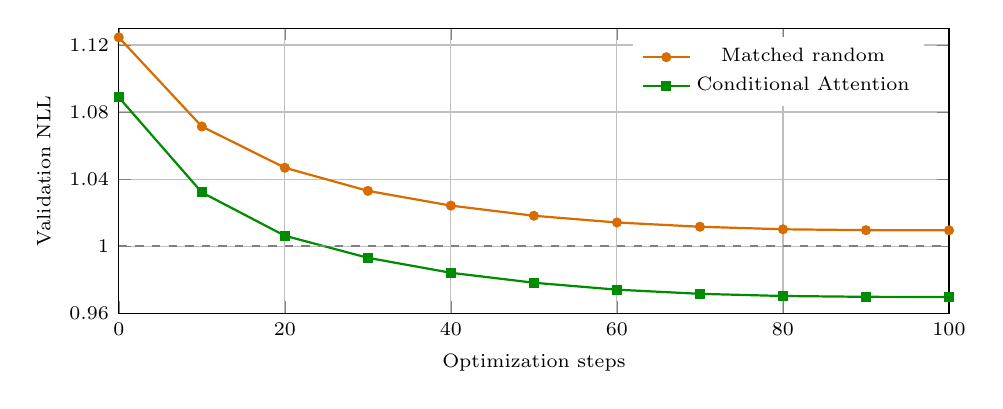
\begin{tikzpicture}
    \begin{axis}[
      width=\columnwidth,
      height=5.2cm,
      xmin=0, xmax=100,
      ymin=0.96, ymax=1.13,
      xtick={0,20,40,60,80,100},
      ytick={0.96,1.00,1.04,1.08,1.12},
      xlabel={Optimization steps},
      ylabel={Validation NLL},
      grid=major,
      tick label style={font=\scriptsize},
      label style={font=\scriptsize},
      legend style={font=\scriptsize, draw=none, at={(0.97,0.97)}, anchor=north east},
      every axis plot/.append style={thick, mark size=1.4pt}
    ]
      \addplot[orange!85!black, mark=*] coordinates {(0,1.12455)(10,1.07137)(20,1.04675)(30,1.03296)(40,1.02416)(50,1.01810)(60,1.01409)(70,1.01155)(80,1.01003)(90,1.00951)(100,1.00941)};
      \addlegendentry{Matched random}
      \addplot[green!55!black, mark=square*] coordinates {(0,1.08880)(10,1.03203)(20,1.00618)(30,0.99302)(40,0.98408)(50,0.97814)(60,0.97400)(70,0.97152)(80,0.97023)(90,0.96973)(100,0.96963)};
      \addlegendentry{Conditional Attention}
      \addplot[gray, dashed, no marks] coordinates {(0,1.0)(100,1.0)};
    \end{axis}
  \end{tikzpicture}
  \vspace{-5pt}
  \caption{Mean matched validation NLL across three adaptation runs. Conditional Attention reaches the fixed NLL threshold earlier and remains below Random throughout training.}
  \Description{A two-line convergence plot over 100 optimization steps. Conditional Attention remains below matched random selection at every checkpoint and crosses NLL 1.0 at step 30.}
  \label{fig:conditional_attention_convergence}
\end{figure}

\paragraph{Answer to RQ3.} At comparable compression, Conditional Attention selects lower-shift occurrences and yields faster, lower-loss adaptation.

\subsection{RQ4: Parameter Sensitivity}
\label{subsec:sensitivity}

Following the one-factor-at-a-time design used by REPFINDER~\cite{repfinder2021}, we vary one decision parameter while holding the others fixed. Because registry capacity determines the vocabulary used during adaptation, we select it on a held-out mixture of engineering code and algorithmic solutions that matches the adaptation domains. Its candidates are mined only from the corresponding training partitions, and the curve uses nested prefixes of one fixed ranking. The remaining mining-bound experiments use the held-out LeetCode split with the Qwen2.5-Coder-1.5B tokenizer and center on $f_{\min}=10$, $W_{\max}=8$, $H_{\max}=6$, and a registry cap of $K=800$; the larger cap prevents registry truncation from hiding differences among these parameters. No test split is used for parameter selection.

In Figure~\ref{fig:parameter_sensitivity}, $K$ is the registry capacity, namely
the maximum number of shorthand entries retained. The minimum support
$f_{\min}$ is the minimum number of occurrences required for a mined pattern
to remain a candidate. The maximum window $W_{\max}$ is the largest local
token or syntax window considered when collecting contiguous patterns. The
maximum captures $H_{\max}$ is the largest number of typed variable,
literal, or expression captures allowed in one generalized pattern. A plateau
means that increasing the parameter further produces negligible additional
token reduction under the fixed evaluation protocol.

\begin{figure*}[!t]
  \centering
  \begin{tikzpicture}
    \begin{groupplot}[
      group style={group size=4 by 1, horizontal sep=0.55cm},
      width=0.235\textwidth, height=3.9cm,
      grid=major,
      tick label style={font=\scriptsize},
      label style={font=\scriptsize},
      title style={font=\footnotesize},
      every axis plot/.append style={blue, thick, mark=*, mark size=1.5pt}
    ]
      \nextgroupplot[
        title={(a) Registry},
        xlabel={$K$}, ylabel={Reduction (\%)},
        xmin=0, xmax=460, ymin=9, ymax=14,
        xtick={0,128,256,384}
      ]
      \addplot coordinates {(0,9.0629)(64,11.2531)(128,12.1151)(192,12.4793)(256,12.7194)(320,12.9382)(384,13.4493)(400,13.5346)(416,13.6067)(432,13.6788)(448,13.7150)(457,13.7312)};
      \addplot[gray, dashed, no marks] coordinates {(448,9)(448,14)};
      \addplot[red!75!black, only marks, mark=star, mark size=2.3pt] coordinates {(443,13.6605)};

      \nextgroupplot[
        title={(b) Support},
        xlabel={$f_{\min}$},
        xmin=5, xmax=40, ymin=16, ymax=22,
        xtick={5,10,20,40}
      ]
      \addplot coordinates {(5,19.6677)(10,21.1094)(20,19.1765)(40,16.9805)};

      \nextgroupplot[
        title={(c) Window},
        xlabel={$W_{\max}$},
        xmin=4, xmax=12, ymin=20.8, ymax=21.25,
        xtick={4,8,12}
      ]
      \addplot coordinates {(4,20.9604)(8,21.1094)(12,21.1085)};

      \nextgroupplot[
        title={(d) Captures},
        xlabel={$H_{\max}$},
        xmin=2, xmax=10, ymin=19.2, ymax=21.3,
        xtick={2,6,10}
      ]
      \addplot coordinates {(2,19.4716)(6,21.1094)(10,21.1094)};
    \end{groupplot}
  \end{tikzpicture}
  \vspace{-5pt}
  \caption{One-factor sensitivity of Hybrid Idioms Shorthanding. Registry capacity $K$, minimum support $f_{\min}$, maximum window $W_{\max}$, and maximum captures $H_{\max}$ are defined in the text. Panel (a) uses the held-out adaptation-domain mixture; the star marks the 443-entry training registry obtained by pruning the 448-entry plateau vocabulary. Panels (b)--(d) use held-out LeetCode.}
  \Description{Four line charts show token reduction against registry capacity, minimum pattern support, maximum mining-window length, and maximum number of typed captures. The registry curve approaches a plateau near 448 entries and marks the deployed 443-entry registry; reduction peaks at support 10 and plateaus at window 8 and capture bound 6.}
  \label{fig:parameter_sensitivity}
\end{figure*}

Figure~\ref{fig:parameter_sensitivity}(a) makes the capacity plateau explicit. Total reduction rises from 9.06\% without idiom entries to 13.45\% at $K=384$, then reaches 13.53\%, 13.61\%, and 13.68\% at $K=400$, 416, and 432. Expanding the registry to 448 and then to the complete 457-candidate vocabulary yields only 13.715\% and 13.731\%, respectively. Thus $K=448$ retains 99.65\% of the maximum shorthand gain, while the final nine entries contribute only 0.016 percentage points. For adaptation, we further remove five entries that are not materialized in at least one of the actual training or validation corpora. The resulting $K=443$ registry retains 98.49\% of the maximum shorthand gain; all 443 symbols occur in the adaptation training corpus, with a median of 56 occurrences and 430 symbols appearing at least ten times.

The mining bounds have clearer interior optima. Setting $f_{\min}=10$ gives 21.11\% reduction, compared with 19.67\%, 19.18\%, and 16.98\% at 5, 20, and 40. Increasing $W_{\max}$ from 4 to 8 improves reduction from 20.96\% to 21.11\%, with no further gain at 12. Likewise, increasing $H_{\max}$ from 2 to 6 improves reduction from 19.47\% to 21.11\%, while 10 produces the same result.

The sensitivity results identify an operating region rather than a universally optimal value. Registry capacity and minimum pattern support have the largest effect, while the window and capture bounds reach an early plateau. We therefore use $(K,f_{\min},W_{\max},H_{\max})=(443,10,8,6)$, which preserves nearly all available compression while avoiding unnecessary vocabulary entries and mining cost.

\paragraph{Answer to RQ4.} \tool is most sensitive to registry capacity and minimum pattern support, while the window and capture bounds enter a stable plateau. Capacity saturates at approximately 448 entries, and exposure-aware pruning produces the 443-entry registry used for mainline adaptation.

\subsection{Ablation Study}
\label{subsec:ablation}

We ablate \tool at its two principal decision boundaries: what is represented compactly by the codec, and where an eligible shorthand is materialized.

\begin{table}[H]
    \centering
    \footnotesize
    \setlength{\tabcolsep}{4pt}
    \renewcommand{\arraystretch}{1.08}
    \caption{Codec-component ablation across the five tokenizers. Values are token-reduction ranges; the Hybrid column reports the additional gain over Normalization.}
    \vspace{-5pt}
    \label{tab:codec_ablation}
    \begin{tabular}{@{}lrrr@{}}
    \toprule
    \textbf{Corpus} & \textbf{Normalization (\%)} & \textbf{Hybrid gain (pp)} & \textbf{Full \tool (\%)} \\
    \midrule
    CodeSearchNet & 5.62--35.53 & +0.58--0.98 & 6.57--36.11 \\
    StarCoder Python & 7.66--34.67 & +0.35--1.69 & 9.35--35.02 \\
    LeetCode & 10.32--48.41 & +4.52--8.81 & 19.13--52.93 \\
    \bottomrule
    \end{tabular}
\end{table}

Table~\ref{tab:codec_ablation} shows that Normalization alone provides the larger and more stable part of the reduction. Adding Hybrid Idioms Shorthanding produces a positive gain for every tokenizer, with the largest contribution on LeetCode. Holding the candidate registry and token-removal level fixed, replacing Conditional Attention with matched random occurrence selection changes cumulative delta-NLL from $-5.03$ to $+2.65$; reversing the learned ordering further increases it to $+8.03$. The final validation NLL rises from 0.9696 with Conditional Attention to 1.0094 with matched random selection, and the random policy does not reach the fixed NLL threshold within the 100-step training run.

The ablation results show that the components address different sources of difficulty. Normalization supplies broadly available structural reduction, Hybrid Idioms Shorthanding captures residual corpus repetition, and Conditional Attention reduces the learning cost introduced by deciding where those idioms are materialized. The three components are complementary rather than interchangeable.


\subsection{Threats and Limitations}

\hspace*{\parindent}\textbf{Threats.} To reduce data leakage, we construct the mining,
calibration, training, validation, and test partitions independently and check
for overlap at the problem-group level. Residual semantic duplication across
independently sourced corpora may nevertheless remain. Our codec measurements
depend on the correctness of the parser, tokenizer integrations, and inverse
transformations; we mitigate this threat with round-trip tests and by counting
fallback inputs in the reported coverage rather than silently excluding them.
Downstream pass rates may vary with training seed and checkpoint selection. We
therefore use a fixed evaluation protocol and report the checkpoint and
condition used for each comparison; broader multi-seed training would further
strengthen these results. Finally, the evaluated corpora, Python syntax, and
model families do not cover every programming language or deployment setting,
so the observed reduction and adaptation behavior should not be assumed to
transfer unchanged beyond the studied configurations.

\indent\textbf{Limitations.} The main codec guarantee is AST-equivalent executable recovery for accepted outputs, not byte-for-byte preservation of formatting or comments. Some inputs still fall back to native Python and remain in the denominator when reporting coverage. RQ1 uses tokenizer- and corpus-specific registries, so it measures capacity rather than universal cross-domain transfer. RQ2 now includes several model families and sizes, but the parallel runs use model-specific adapters and should be interpreted as within-backbone comparisons rather than a ranking of base models. RQ3 uses a fixed candidate subset from one primary calibration domain. Offline attention scoring also adds a preprocessing cost. Future evaluation should test whether the same selection principle transfers to additional programming languages and longer-context tasks.
